\documentclass[12pt]{article}
% 12pt font size, article class.
% Usually stick to this, though you can try "amsart" for an AMS style article instead.

\usepackage{amsmath,amssymb,psfrag,epsfig,boxedminipage,helvet,amsthm,endnotes,version,multicol}
\usepackage{pgfplots}
\usepackage{tikz}
\usetikzlibrary{automata, positioning, arrows}
% Package imports. We probably don't need all of them, but it doesn't hurt.

\title{Problem Set 4}
\author{Your Name Here!}
\date{}

\makeatletter
\let\newtitle\@title
\makeatother

\renewcommand{\thepage}{\footnotesize MAT 4520, Computability, \newtitle, p. \arabic{page}} 

\newcommand{\sol}{\par{\bf SOLUTION}: }

\begin{document}

\maketitle

\noindent
    {\bf Due: Monday 4/22, at 11:59pm. }
    
\begin{enumerate}
	
\item Show that $A_{TM} \leq_T \overline{A_{TM}}$ and $\overline{A_{TM}} \leq_T A_{TM}$. That is, show that $A_{TM}$ is Turing-equivalent to its complement. (Note: These are \emph{Turing reductions}, not $m$-reductions!)

\sol % Put your solution here!

\item Sketch a proof that the class $P$ is closed under intersection and complements.

\sol % Put your solution here!

\item Recall the language $FIN$ defined by:
\begin{displaymath}FIN = \{ \langle M \rangle : \mathcal{L}(M) \text{ is finite } \}.\end{displaymath}

Show that $A_\textrm{TM} \leq_\text{m} FIN$. (Hint: given $\langle M, w \rangle$, we construct a machine $M^\prime$ so that, on input $x$, $M^\prime$ should run $M$ on input $w$ for $|x|$ steps. What should $M^\prime$ then do if $M$ accepts in that many steps? What if $M$ does not accept in that many steps?)

\sol % Put your solution here!

\item Let $G = (V, E)$ be a finite graph. An \textit{Eulerian path} is a path through the graph which visits every edge exactly once. An \textit{Eulerian circuit} is an Eulerian path that begins and ends at the same vertex. A graph is called \textit{Eulerian} if it has an Eulerian circuit. Let $E = \{ \langle G \rangle : G$ is an Eulerian graph $ \}$. Show that $E \in P$.

(Hint: Every time you visit a vertex, you have to enter it through one edge and leave it through another. What does that tell you? Is the following graph Eulerian? Why or why not? Is there an edge you can delete that makes it Eulerian?)

\begin{center}
	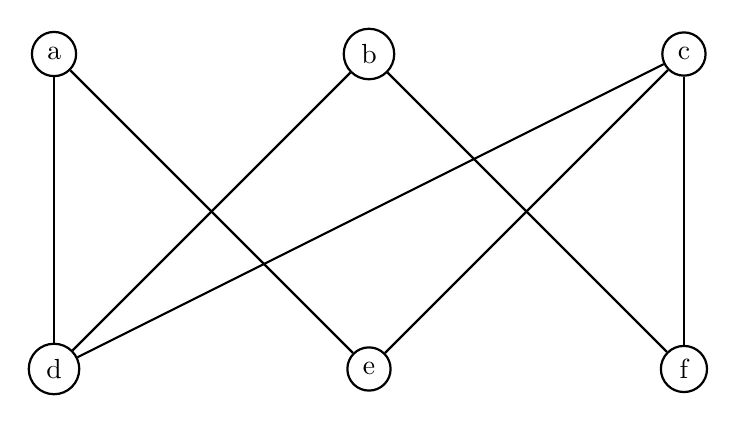
\begin{tikzpicture}[node distance=40mm, thick, main/.style = {draw, circle}, baseline=(current bounding box.north)] 
	\node[main] (a) {a};
	\node[main] (b) [right of=a] {b};
	\node[main] (c) [right of=b] {c};
	\node[main] (d) [below of=a] {d};
	\node[main] (e) [below of= b]{e};
	\node[main] (f) [below of=c] {f};
	\draw (a) -- (d);
	\draw (b) -- (d);
	\draw (c) -- (d);
	\draw (a) -- (e);
	\draw (c) -- (e);
	\draw (b) -- (f);
	\draw (c) -- (f);
	\end{tikzpicture}
\end{center}

\sol % Put your solution here!

%%% LaTeX HINTS:

% If you want to "draw" diagrams in LaTeX, you have two options:

%1. Use tikz. This can be hard, but you can look at the example from Pre-Work Lesson 2, copied over here.
%	\begin{figure}[ht]
%	\centering
%	\begin{tikzpicture}
%	\node[state, initial] (q0) {$q_0$};
%	\node[state, right of=q0] (q1) {$q_1$};
%	\node[state, accepting, right of=q1] (q2) {$q_2$};
%	\draw (q0) edge[above] node{0, 1} (q1)
%	(q1) edge[above] node{0, 1} (q2)
%	(q2) edge[bend left, below] node{0, 1} (q0);
%	\end{tikzpicture}
%	\end{figure}

%2. Draw it by hand. Take a good picture, crop it, and upload it to overleaf. Then use the following command:

% \includegraphics{filename-without-extension}
% Depending on the dimensions of the picture, you might need to rescale it:
% \includegraphics[scale=0.5]{filename-without-extension}.
% Sometimes I need to use scale=0.2 or 0.3 before the pictures display decently.

\end{enumerate}

\end{document}